\documentclass[figure,letterpaper,onefignum]{mysiam}

%%%
% packages
%%%
\usepackage{amssymb}
\usepackage{amsmath}
\usepackage{float}
\usepackage{pifont}
\usepackage{graphicx}
\usepackage{caption}


%%%
% new commands
%%%
\newcommand{\sm}[1]{\mathcal{#1}}
%\newcommand{\tld}[1]{\tilde{#1}}
\newcommand{\bo}[1]{\mathbf{#1}}
\newcommand{\bx}{\mathbf{x}}
\newcommand{\br}{\mathbf{r}}
\newcommand{\floor}[1]{\left\lfloor#1\right\rfloor}
\newcommand{\ceil}[1]{\left\lceil#1\right\rceil}
\newcommand{\real}{\mathbb{R}}
%\newcommand{\ra}{\rightarrow}
\newcommand{\bt}[1]{\textcolor{blue}{#1}}
\newcommand{\rt}[1]{\textcolor{red}{#1}}
%\newcommand{\E}{\text{E}}
\newcommand{\rk}{r^{(k)}_{nm}}
\newcommand{\red}{\color[rgb]{1,0,0}}

\newcommand{\term}[1]{{\textbf{\textit {#1}}}}

%%%
% declarations
%%%
\DeclareMathOperator{\prob}{Prob}
\DeclareMathOperator{\cov}{Cov}
\DeclareFontFamily{U}{msb}{}
\DeclareFontShape{U}{msb}{m}{n}{ <5> <6> <7> <8> <9> gen * msbm
  <10> <10.95> <12> <14.4> <17.28> <20.74> <24.88> msbm10}{}
\DeclareSymbolFont{AMSb}{U}{msb}{m}{n}
\DeclareMathSymbol{\E}{\mathalpha}{AMSb}{"45}
\newcommand{\zig}{\Pisymbol{psy}{126}}
\setlength{\parskip}{10pt}
\setlength{\parindent}{0pt}

%%%%%%%%%%%%%%%%%%%%%%%%%%%%%%%%%%%%%%%%%%%%%%%%%%%%%%%%%%%%%%%%%
%% title stuff
%%%%%%%%%%%%%%%%%%%%%%%%%%%%%%%%%%%%%%%%%%%%%%%%%%%%%%%%%%%%%%%%%
\title{Toward Type Safety in Programming Languages for Penetration Testing}

\author{Isaac Potoczny-Jones \and
  Trevor Elliott, Galois, Inc \thanks{PROPRIETARY DATA \copyright 2013 Galois, Inc. - For information contact \email{ijones@galois.com}}
}

%%%
% document starts
%%%
\begin{document}

\maketitle

%%%%
% ABSTRACT
%%%%
%\begin{abstract}
%Abstract here.
%\end{abstract}

%%%
% keywords if necessary
%%%

%\begin{keywords}
%topic1, topic2, topic3
%\end{keywords}

%%%
% page style stuff
%%%
\pagestyle{myheadings}
\thispagestyle{plain}

%%%
% page markings
%%%
\markboth{Toward Type Safety in Programming Languages for Penetration Testing}{Toward Type Safety in Programming Languages for Penetration Testing}
%%%
% body - use section, subsection, and paragraph tags for different parts of
% the text.
%%%

\section{Introduction}
In this whitepaper, we discuss Tuna, a prototype tool for improving the safety of automated penetration testing through the use of a programming language type system. We have successfully implemented a prototype domain-specific library for penetration tests that includes strong type checking that can help developers avoid a wide range of programming errors.

Penetration testing automation is becomming more common, but this comes with the risk of unintentionally damaging systems through programming errors. This is particularly true as automated tools become more complex. This is a trend that is likely to continue, and it's important to build tools that support both complexity and correctness.  To support complexity, Tuna provides the full power of a general purpose programming language (Haskell). To support improved correctness, it includes strong type safety as well as domain-specific concepts for penetration testers.

Penetration testing always involve the risk of unintended damage to systems due to user error or defective tools. This risk is even greater when testers increase automation through the use of programming languages that attempt to coordinate complex interactions among tools that humans normally coordinate by hand. Furthermore, automated tools can be more clumsy or brute-force than a human would be, causing a high volume of suspicious network traffic.

Building correct software is well known to be a difficult task, and it's very likely that automated penetration testing tools will have programming errors. Such errors can be benign or they can cause serious damage. For instance, even unobtrusive actions like port scans sometimes crash fragile systems.

For this reason, penetration testing is typically done with significant human involvement. Those systems that do not involve humans, such as automated scanning and exploitation systems that build botnets, are most likely unconcerned with collateral damage, or even detection.

The Metasploit Framework (MSF), produced by Rapid7 LLC, is a penetration testing toolkit with capabilities like scanning a network to detect hosts (using the network mapping tool nmap), launching attacks against vulnerable hosts, encoding payloads to avoid detection, and deploying payloads with a wide variety of features for controlling an exploited host. Metasploit has an open source version and a professional version. Tuna currently integrates with the open source version.

Cortana is a related open source tool that's integrated into the Cobalt Strike product by Strategic Cyber LLC. It is a domain-specific programming language that allows for scripting of the Metasploit Framework. This innovative language can help to control and coordinate Metasploit's many capabilities, allowing a penetration tester to automate complex but repeatable tasks. Cortana has features where a developer can increase the safety of the system by adding hand-coded run time correctness checks. Cortana is designed to work similarly to a \emph{scripting} language such as Perl, which allows a developer to quickly glue together functionality and get a program working, but offers very few language features to ensure correctness and safety of the developed code. 

Our approach is Tuna: a domain-specific language embedded in Haskell for controlling Metasploit that includes improved program correctness checking. It accomplishes this through the use of Haskell's type system. Our tool implements most of the major features of Cortana: Complete control of Metasploit and event handling. Our tool also offers improved type safety and higher-level abstractions that are not available in Cortana. On the other hand, Cortana can also be used to extend and control Armitage, a Metasploit GUI front-end; we have no plans to support this capability.  We have also not yet added support for locking (coordination among multiple instances of our tool) or notification in the shared event log.

\section{Types of Programming Errors}
Programming languages can be characterized by the levels of abstraction that are provided to the developer. Binary and assembly languages are very low level and provide very little abstraction. Higher-level languages allow the programmer to build data types that more closely represent the domain they are operating in. We consider several types of programming errors that can cause collateral damage, and demonstrate how higher-level languages like Haskell provide an advantage over lower-level languages like Perl in preventing errors at different abstraction levels.  In each case, we are able to detect errors at compile time that would otherwise not be detected at all, or only detected at run time under certain circumstances. For examples of these errors and how they are addressed by Tuna, see Appendix \ref{secExampleErrors}.

\subsection{Compile time errors verses run time errors}
For most of the errors described in this section, it is possible to detect them either statically at compile time or dynamically at run time. Detecting errors at compile time is usually better, particularly for software that can cause damage.

Languages without strong typing can sometimes detect errors at run time, even if they are unable to detect them at compile time. To detect a run time error, the developer needs to find a test case that exercises the error. This can be difficult when the error happens only in rare circumstances, and so many such errors go undetected. Even if the developer does have such a test case, run time errors can have a wide variety of behaviors: They can cause the program to exit with an error code and print an error message, they can continue with or without an error message, or they can do the wrong thing in a manner undetectable by the developer.

In contrast, compile time errors are always detected without testing. In our library design, our goal was to use domain-specific knowledge to detect programming errors at compile time.

\subsection{Basic semantic and typographical errors}
At the lowest level of abstraction, we consider basic semantic errors. These are errors where the developer uses the language incorrectly or makes simple typographical mistakes. This can include using the wrong name for a function, passing the wrong number of parameters, forgetting to import a library, etc.

In most languages like C, Java, and Haskell, these errors are detected at compile time. In other languages, it's not possible to determine statically whether or not these are errors, and they are likely to cause the program to crash, behave incorrectly, or output an error message.

Since Tuna is implemented within the Haskell language, such errors are detected at compile time.

\subsection{Type errors - Distinguishing by form}
At a higher level of abstraction, a programmer can confuse symbols that have completely different forms and representations. A simple example is using a String where an Integer was expected. All Integers can be converted to Strings, but not vice-versa.

In most languages like C, Java, and Haskell, these errors are detected at compile time. In some languages, types like Integers and Strings are automatically coerced (converted) at runtime, potentially causing the program to crash if coercion is not possible. 

Even with language support for strong typing, it's possible to program without taking advantage of types. For instance, the IP address of hosts is often a parameter to functions in Metasploit. This address can be represented as a String, or the programmer could create a custom type that's distinct from a String. Similarly, an Exploit can be represented by its name (a String) or the programmer can create a distinct type. If the programmer does create these types, they will get a compile time error if they mix up a Host with an Exploit. If not, they won't get an error until run time.

We found at least one example in Metasploit where Job IDs were treated inconsistently, sometimes as Integers and sometimes as Strings. In another case, the Metasploit API documentation instructs users to be careful not to assume that Console ID Strings will always be valid Integers. Strong typing helps to eliminate such issues.

In Tuna, we have distinguished among a large number of types that are all represented by Strings in Metasploit and Cortana: Hosts, Tokens, Job IDs, Console IDs, Payloads, Modules, and various other types are all distinct. In practice, this has helped us as programmers when we have used the wrong symbols in certain places.

\subsection{Type errors - Distinguished by use and phase of attack}
The above errors involve types that had completely different forms and representations. However, sometimes two conceptually different types have the same form and representation. For instance, the developer could mix up two different ``kinds'' of hosts or mix up JobIDs with Console IDs. These errors won't be detected at compile time and might not even be detected at run time. Increased knowledge of the domain is required to prevent these errors.

Mixing up different kinds of hosts is a particularly worrying error. The user could accidentally launch an attack against the Metasploit server itself, or against a DNS server that they had meant to query. At a somewhat higher level of abstraction, these distinctions might occur at different phases of an attack. During a particular phase, it might be the user's intention to only scan a host with nmap, not to attack it with an exploit, but through a programming error, the developer might mix up the hosts.

Without explicit support, these errors are highly unlikely to be detected at run time. For instance, an attack against the Metasploit server might simply fail, but this won't necessarily be surprising since attacks against legitimate targets often fail. Similarly, attacking a host that the user meant to only scan could cause it to crash. If this target was a sensitive server that the penetration tester was told not to attack, they will have some explaining to do.

In Tuna, we distinguish between different host types: The Metasploit server, Scannable hosts, and Attackable hosts. This can help to prevent the user from accidentally launching attacks against the wrong server.

\subsection{Attack Loudness Constraints}
Another differentiation we might like to make in different phases of a penetration test the ``volume'' of the attack, that is whether an operation is loud or quiet. It can sometimes be problematic to generate a lot of suspicious network traffic, but at other times it is not problematic or it is unavoidable.

Without explicit support, programming errors of this kind are unlikely to be detected at run time, at least by the penetration tester. They might instead be noticed by an IDS. This could result in the tester's IP address being blocked and subsequent tests to fail.

For each function in Tuna, we provide a ``volume context'' parameter stating whether the function is ``Silent'', ``Quiet'' or ``Loud''. The meaning of these types is arguable, and certainly depends on the type of penetration test being performed. We offer these definitions:

A \emph{silent} operation is one which interacts with the Metasploit server, but does not itself directly cause any action that interacts with a target. For example, logging into the Metasploit server or listing open sessions.

A \emph{quiet} operation \emph{can} impact a target, like closing a session if one is already open, and some types of "quiet" port scans. In practice it might be that with modern defenses, even quiet port scans are easy to detect.

A \emph{loud} operation is one which seems to us would likely be detected by an IDS. This includes loud nmap scans and launching exploits. Of course, some modules are probably quiet.

If a function calls a loud function, the calling function inherits the loud function's ``volume context''. A loud function cannot be called from a quiet context, but a quiet function can be called from a loud context. Silent functions can be called from any context. These properties are enforced by the type system, but the user can choose to override them explicitly.

\section{Conclusion}
Programming errors can have an impact on the collateral damage caused by a potentially dangerous tool like the Metasploit Framework. Without explicit support, such errors will not be detected by the compiler before running the code and might not even be detected by the run time system. With knowledge of the domain, a programming language designer or library designer can use strong typing to detect such errors at compile time, significantly reducing the likelihood of collateral damage.

We have implemented a domain-specific language called Tuna which includes a wide variety of such compile time checks. The API we provide includes domain-level concepts like different types of hosts and different phases of attack that can be used by a developer to not only avoid low-level errors like mixing up integers with strings, but domain-level errors like accidentally launching a loud port scan when a quiet scan was more appropriate. Strong typing encourages the programmer to have a clear mental model of the system, and so compilation can be a ``quality gate'' that shows that a large class of basic mistakes have been avoided.  

Similar to other high-level programming languages like Java, Haskell provides the ability to build complex abstractions and data structures. This allows developers to work with a larger code base. Also, Haskell is a widely-used programming language with thousands of libraries available. Building our system as a library within Haskell rather than a stand-along programming languages means that we can use the full power of the language and the libraries.

Untyped scripting languages have some advantages over strongly typed languages. Untyped scripting languages like Perl and Cortana are powerful and easy to use. In such languages, it's easy to get a minimal system up and running quickly. The compile, run, debug loop is fast since compilation checks are largely left out, and so the programmer can quickly see the results of their changes.

Programmers can write bad code or good code in any programming language, but the language can provide programmers with tools to write better code if it is important enough. For potentially dangerous tools like automated penetration testing frameworks, we argue that the trade-off between correctness and ease-of-use depends on the situation. For small and quick penetration tests with a human monitoring the behavior of the system, a scripting language is highly appropriate.  For large, complex, autonomous, and sensitive work, we would prefer to use a strongly-typed language with high-level abstraction capabilities.

\appendix
\section{Example Programming Errors and Compile Time Detection}
\label{secExampleErrors}
\subsection{Reading Type Signatures}
In this section, we describe several functions and values that are \emph{strongly typed}, meaning that there is compile time enforcement of their allowable values. We make extensive use of \emph{type signatures} that describe the types. Type signatures in this section are often simplified in comparison to the practical API design outlined in the next section. By way of a brief introduction to type signatures, we offer a few examples:

\begin{verbatim}
numberOfExploits :: Integer
\end{verbatim}

The symbol double-colon should be read ``has the type'', so the above type signature reads ``the symbol \emph{numberOfExploits} has the type \emph{Integer}''.

In type signatures, function parameters are separated by arrows, and the element after the last arrow is the return value.

\begin{verbatim}
launch :: Exploit -> Host -> Payload -> IO (Maybe Session)
\end{verbatim}

This should be read ``The function \emph{launch} takes three parameters, an \emph{Exploit}, a \emph{Host}, and a \emph{Payload}. It performs \emph{IO} actions and maybe returns a \emph{Session} (or maybe returns \emph{Nothing})''.

\subsection{Basic semantic and typographical errors}
As with many scripting languages, Cortana does not check whether symbols (e.g. function calls) correctly map to a known function at compile time. For instance, a programmer can call a function that does not exist, and this error will not be caught by the interpreter unless and until the code in question is executed:

\begin{verbatim}
println ("This println function call is correct.");
print ("The print function doesn't actually exist."); #run time error
\end{verbatim}

\subsection{Type errors - Distinguishing by form}
A developer might provide parameters to functions that are ill-formatted for their type. The extensive use of strings for most parameters in Cortana means that the programmer can provide a parameter for the ``exploit'' type when they wanted to provide a parameter of the ``host'' type. These can be detected at run time during serialization or use of the type. Such errors are not specific to scripting languages; any programming language can have an API designed in this manner.

Consider a function ``launch'' that launches a given exploit against a host and if successful, returns a session that the programmer can interact with. (See the ''launch'' function in Cortana.) In practice, this function is asynchronous, but for clarity, we provide a type that appears to return immediately. The Cortana language does not use different types for things like hosts, exploits, payloads, etc, these are strings. A function type, and an example function call demonstrating this problem might look like this:

\begin{verbatim}
launch :: String -> String -> String -> IO (Maybe Session)

-- function call context

let exploit = "ms08_067"
let targetHost = "192.168.95.166"
let payload = "bind_tcp"
...
session <- launch exploit targetHost payload -- Correct
\end{verbatim}
Since the parameters are all the same String type, the developer can accidentally provide incorrect parameters to this function without triggering a compile time error. This could happen by providing the parameters in the incorrect order or providing the wrong kind of parameter altogether:

\begin{verbatim}
session <- launch targetHost exploit payload -- Run Time Error: wrong order
session <- launch exploit targetHost "anything goes"
           -- Run Time Error: wrong kind of string
\end{verbatim}
With good API design, this type of problem is easily detected at compile time in a typed language like Haskell or Java since function calls can be designed to expect particular types. For instance, an example function type definition and call might look like this:

\begin{verbatim}
launch :: Exploit -> Host -> Payload -> IO (Maybe Session)

-- function call context:

let exploit = Exploit "ms08_067"
let targetHost = Host "192.168.95.166"
let payload = Payload "bind_tcp"
...
session <- launch exploit targetHost payload -- Correct
session <- launch targetHost exploit payload -- compile time Error
\end{verbatim}

\subsection{Type errors - Distinguished by use}
In the following example, the client-side script has to connect to the Metasploit server (one kind of host) and instruct the Metasploit server to launch an attack against a target (another kind of host):

\begin{verbatim}
let metasploitServer = Host "127.0.0.1"
let targetHost       = Host "192.168.95.166"

-- function call context:

connect :: Host   -> IO (Handle)
launch  :: Handle -> Exploit -> Host -> Payload -> IO (Maybe Session)

h <- connect metasploitServer
launch h exploit targetHost payload -- Correct
\end{verbatim}
Since both the Metasploit server host and the target host are of the same ''Host'' type, it is possible for a developer to mix up these parameters and accidentally launch an attack against the Metasploit server itself. This would not be caught at compile time, since it's not a type error (they are both Hosts, after all) and an error is unlikely to be thrown at run time. The error might not be detected unless a human penetration tester notices the problem.

\begin{verbatim}
launch h exploit metasploitServer payload -- Error: might never be detected
\end{verbatim}
This can be corrected by using different types for these very different uses of hosts:

\begin{verbatim}
connect :: ServerHost -> IO Handle
launch  :: Handle -> Exploit -> TargetHost -> Payload -> IO (Maybe Session)

-- function call context:

let metasploitServer = ServerHost "127.0.0.1"
let targetHost       = TargetHost "192.168.95.166"

launch h exploit metasploitServer payload -- compile time Error
\end{verbatim}
Notice that these types now include a higher-level understanding of the domain and what kinds of actions are desirable in the domain. This Haskell binding to Metasploit allows us to capture domain-specific concepts and prevent higher-level conceptual errors.

\subsection{Type errors - Distinguished by phase of attack}
During the ``discovery'' phase of an attack, the penetration tester might launch scans with nmap, which detects live hosts and open ports on those hosts. The discovery phase might be relatively quiet to avoid detection. Once hosts are discovered, specific target hosts are selected, and the attack moves to the ''exploit'' phase. It's not typical to launch an exploit against all discovered hosts since this can cause collateral damage and cause a large amount of suspicious network traffic.

Through a programming error, a developer could accidentally launch an attack against a host that they wished to only run a quiet scan on. In another phase of the attack, it would be perfectly fine to launch an attack against these hosts, but in the current phase of the attack, it's dangerous and inappropriate. The error cannot be detected by the compiler or by the run time system, although the developer can always add explicit run time checks to detect such errors.

\begin{verbatim}
launch  :: Handle -> Exploit -> TargetHost -> Payload -> IO (Maybe Session)
scanPorts     :: TargetHost -> IO [Port]
hostToScan    :: TargetHost
hostToExploit :: TargetHost

-- function call context:

launch h exploit hostToScan payload
-- Undetected error: Should have run the scanPorts function, not launch
\end{verbatim}
Preventing this class of error requires more domain knowledge to be built into the language. One way to address this error is for the ''launch'' function and the ``scanPorts'' function use different ``Host'' types, as we did in the previous example for the ``ServerHost'' and ``TargetHost'' types.

\begin{verbatim}
launch :: Handle -> Exploit -> ExploitableHost
                 -> Payload -> IO (Maybe Session)
scanPorts     :: ScannableHost -> IO [Port]
hostToScan    :: ScannableHost
hostToExploit :: ExploitableHost

-- function call context:

launch h exploit hostToScan payload
-- compile time error: called "launch" against scanning hosts
\end{verbatim}
Another approach is to use \emph{monads} to force the developer to be explicit about what phase of the attack they are in. The API could provide a set of functions that are each scoped to a particular phase:

\begin{verbatim}
discoverHosts :: IPRange       -> DiscveryPhase [ScannableHost]
scanPorts     :: ScannableHost -> DiscoveryPhase [Port]
launch        :: Handle
              -> Exploit
              -> ExploitableHost 
              -> Payload
              -> AttackPhase (Maybe Session)
\end{verbatim}
Each function that the developer implements would have a matching type that indicates not only the input and output values, but also the phase of the attack (DiscoveryPhase / AttackPhase).

\begin{verbatim}
hostToScan    :: ScannableHost
hostToExploit :: ExploitableHost

-- function call context:

performScansAndReport :: DiscoveryPhase ()
perfromScansAndReport = do
  ports <- scanPorts hostToScan
  putStrLn $ "Open ports: " ++ show ports
  launch handle exploit hostToExploit payload
         -- compile time Error: no exploits allowed in this function
\end{verbatim}
The API can provide a method to override these restrictions, to ``lift'' a function from the DiscoveryPhase to the AttackPhase. For safety, the developer will have to call this explicitly. A similar approach can be used for phases of the attack that might need to be quiet.

\subsection{Attack Volume Constraints}
For instance, the following three functions each have a different ``context''. Logging into the Metasploit server is Silent since it doesn't contact a target. Performing a TCP ``syn'' scan is Quiet since it contacts a target, but tries to be unobtrusive. Performing a TCP ``connect'' scan is Loud.
\begin{verbatim}
auth_login     :: Server -> String -> String -> SilentCxt LoginResult
tcpSynScan     :: Target -> QuietCxt [Ports]
tcpConnectScan :: Target -> LoudCxt [Ports]
\end{verbatim}

A user might decide that the tcpSynScan is not quiet enough for their purposes and provide a wrapper function that changes its context to Loud. Similarly, a user might decide that in a certain circumstance, the tcpConnectScan can be considered quiet. The following two user-defined functions coerce the types to match user preference:

\begin{verbatim}
 -- type coercion is from Quiet to Loud is implicit
loudSynScan :: Target -> LoudCxt [Ports]
loudSynScan t = tcpSynScan t

-- type coercion from Loud to Quiet needs to be done explicitly
quietConnectScan :: Target -> QuietCxt [Ports]
quietConnectScan t = makeQuiet (tcpConnectScan t) 
\end{verbatim}

Users can now build up functionality in any of the various contexts, Silent, Quiet, or Loud. The type system will automatically derive the appropriate context and provide compile time type errors if they have made a mistake:

\begin{verbatim}
-- An example user-defined Loud function that scans all the given targets
myScanningFunction :: [Target] -> LoudCxt ()
myScanningFunction [] = return ()
myScanningFunction (target:rest) = do
  -- auth_login is Silent
  auth_login myServer "username" "password"
  -- tcpSynScan is Quiet
  ports1 <- tcpSynScan target
  if (null ports1) then do
    -- A quiet scan didn't work, use louder scan
    ports2 <- tcpConnectScan target
    print ports2
  else print ports1
  myScanningFunction rest
\end{verbatim}

\section{Tuna API Design}
Many of the above examples are simplified from the types used in the actual API we designed. In this section, we discuss the design of the practical API.

\subsection{Layering}
We provide two layers in the API. The first layer is the ``raw'' RPC layer that implements the procedures in the Metasploit Server with small abstraction improvements. This layer includes some improved type safety over the use of raw strings and (name, value) maps for various elements: Hosts, Tokens, SessionIDs, Consoles, Sessions, etc.

The second layer is a monadic layer called ``MSF'' that raises the abstraction layer significantly. This layer captures relevant state, includes stronger type constraints, handles events, and provides some higher-level functionality for scanning. The MSF layer is implemented in terms of the RPC layer. The user can write code using either layer, but we anticipate that the MSF layer will be easier and safer to use.

In the future, the MSF layer's state can be extended with host blacklists (those hosts not to attack) or similar domain-specific capabilities.

\subsection{Volume context and host types}
We implement SilentCxt, QuietCxt, and LoudCxt as classes and use appropriate instances to allow automatic coercion between them. We also implement various Host types: Server, Attackable and Scannable. Therefore, some functions will have a number of class constraints.

\emph{db\_nmap} is used to construct specific scans. The given target must be scannable (not e.g. the Metasploit server). This function doesn't explicitly constrain the loudness type; it's determined by the nmap options provided.

The user-level function \emph{connectScan} thus has two type constraints: the target host has to be Scannable and the volume context is Loud since it's a very loud kind of port scan.

\begin{verbatim}
db_nmap :: ScanCxt t => NmapOptions s -> Target t -> MSF s ()
tcpConnectScan :: LoudCxt s => NmapOptions s

connectScan :: (LoudCxt s, ScanCxt t) => Target t -> MSF s ()
connectScan = db_nmap tcpConnectScan
\end{verbatim}

Since nmap can take a number of options and each option might impact the volume, we allow them to be combined together. The volume context is automatically derived by the type system based on those parameters:

\begin{verbatim}
-- Has to be loud since tcpConnectScan is Loud:
synAndConnectScan :: (LoudCxt s, ScanCxt t) => Target t -> MSF s ()
synAndConnectScan = db_nmap (tcpSynScan <> tcpConnectScan)
\end{verbatim}


\subsection{Capturing State}
We provide a monad called \emph{MSF} which can be run after logging into a the Metasploit server and receiving an authentication token. This monad captures both the server host and the token so the user does not have to pass these parameters to every single function in the API. The API user also does not have access to the sensitive authentication token, so it is harder to accidentally leak it. The monad also opens a console on the server for ``raw'' console commands.

Functions in the (lower) RPC layer have longer types that include the Metasploit server, the token, and sometimes a console ID:

\begin{verbatim}
session_list  :: Con Server -> Token -> IO SessionList
console_write :: Con Server -> Token -> ConsoleId -> String -> IO Int
\end{verbatim}

In the MSF layer, these have fewer parameters and also include the volume context (Quiet) as a class parameter. Furthermore, console\_write has no volume context, so it can be used in any context, making it a somewhat dangerous function.
\begin{verbatim}
session_list :: (QuietCxt s) => MSF s R.SessionList
console_write :: String -> MSF s ()
\end{verbatim}

To enter the MSF monad, we provide the ``login'' function that takes a username and password, and the MSF computation to be performed. The default volume context is ``Quiet'':

\subsection{Event Handling}
Since many actions in the API are asynchronous or long-running, Cortana uses an event management framework. We have implemented a similar capability. For instance, a user might call db\_nmap, which scans a network and adds any discovered hosts to the Metasploit internal database. For any host discovered, they might want to try launching a particular exploit. To support such a use, each time a host is added, we fire an onHost event. Users can add handlers for this event:

\begin{verbatim}
-- A user-defined function that e.g. attacks any host that's passed to it
attackAllHosts :: (LoudCxt v) => HostInfo -> MSF v ()
-- In the main function, register the handler
onHost attackAllHosts
\end{verbatim}

There are a number of threads that periodically poll for new hosts, service, loot, sessions, or credentials, and the user can register any number of handlers for these events.


\section{Demonstration Environment}
We have built a demonstration environment that includes the following major components as depicted in Figure \ref{archFig}:
\begin{itemize}
  \item MSF: This is the Metasploit Framework, including the server, exploits, payloads, and all Metasploit functionality. This is hosted on a virtual machine running BackTrack, a Linux distribution that is specialized for penetration testing.
  \item Postgres DB: This is a database used by Metasploit to save information during penetration tests. This can include data such as the IP addresses of discovered hosts, the credentials captured, etc. This is hosted on the same BackTrack host as Metasploit, but it can be hosted on a different machine.
  \item Armitage GUI: This is a graphical front-end to Metasploit that we can use for visualization of the data stored in the Postgres DB. It integrates with Metasploit through the Metasploit Server. This is hosted on the same BackTrack host as Metasploit, but it can be hosted on a different machine.
  \item Haskell Tuna: This is the API we developed in the Haskell programming language to control MSF. It interfaces with Metasploit over HTTP. This is running on an Ubuntu Linux development machine.
  \item Target Hosts: These are test systems that are known to be vulnerable to attack and that can be exploited by Metasploit. In particular, we used a virtual machine running the ``Metasploitable'' virtual environment.
\end{itemize}

\begin{figure}[h!]
  \caption{Demonstration Architecture.}
  \label{archFig}
  \centering
    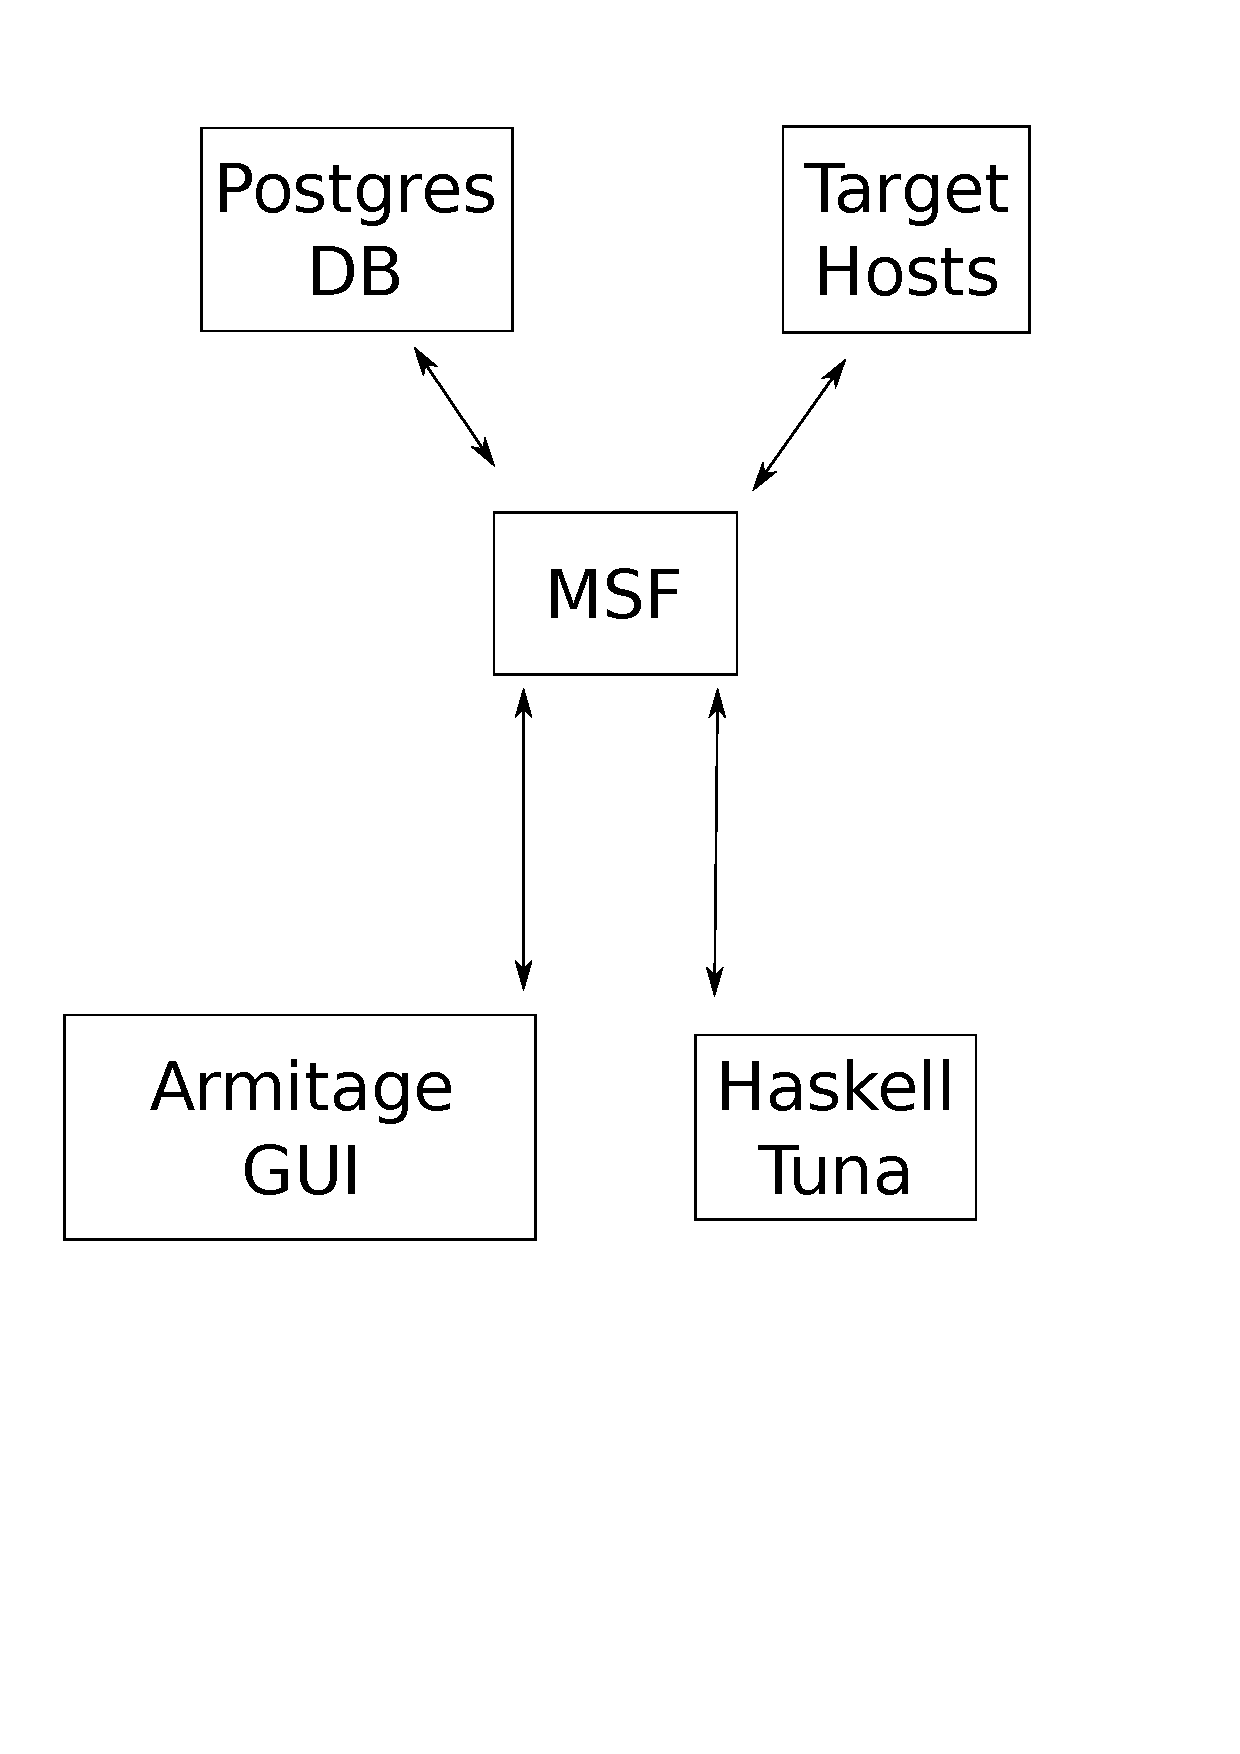
\includegraphics[scale=0.3]{components.pdf}
\end{figure}


As depicted in Figure \ref{dataFlowFig}, these components interact in a relatively complex way, with the Tuna system coordinating the high-level functionality. Tuna initiates nmap scans against the target hosts. This nmap function runs on the same server as MSF, and once nmap discovers hosts, MSF writes the host data such as IP addresses into its database. Then through polling, clients like Tuna and Armitage can be notified of new hosts. Once Tuna receives its notification, it attacks the discovered host. Once Armitage receives its notification, it updates the display to show a discovered host.

Similarly, when Tuna initiates an attack, the attack is launched from MSF, and if successful, the session information is written to the database and Tuna and Armitage are notified. Armitage then displays lightning bolts around the successfully attacked host to indicate that it's been exploited. Once Tuna receives its notification, it fires an event to launch the ``whoami'' program on the target. This is relayed through MSF, and the expected result is ``root''. This indicates that the target is under complete control of Tuna.

\begin{figure}[h!]
  \caption{Example Data Flow Between Major Architectural Components.}
  \label{dataFlowFig}
  \centering
     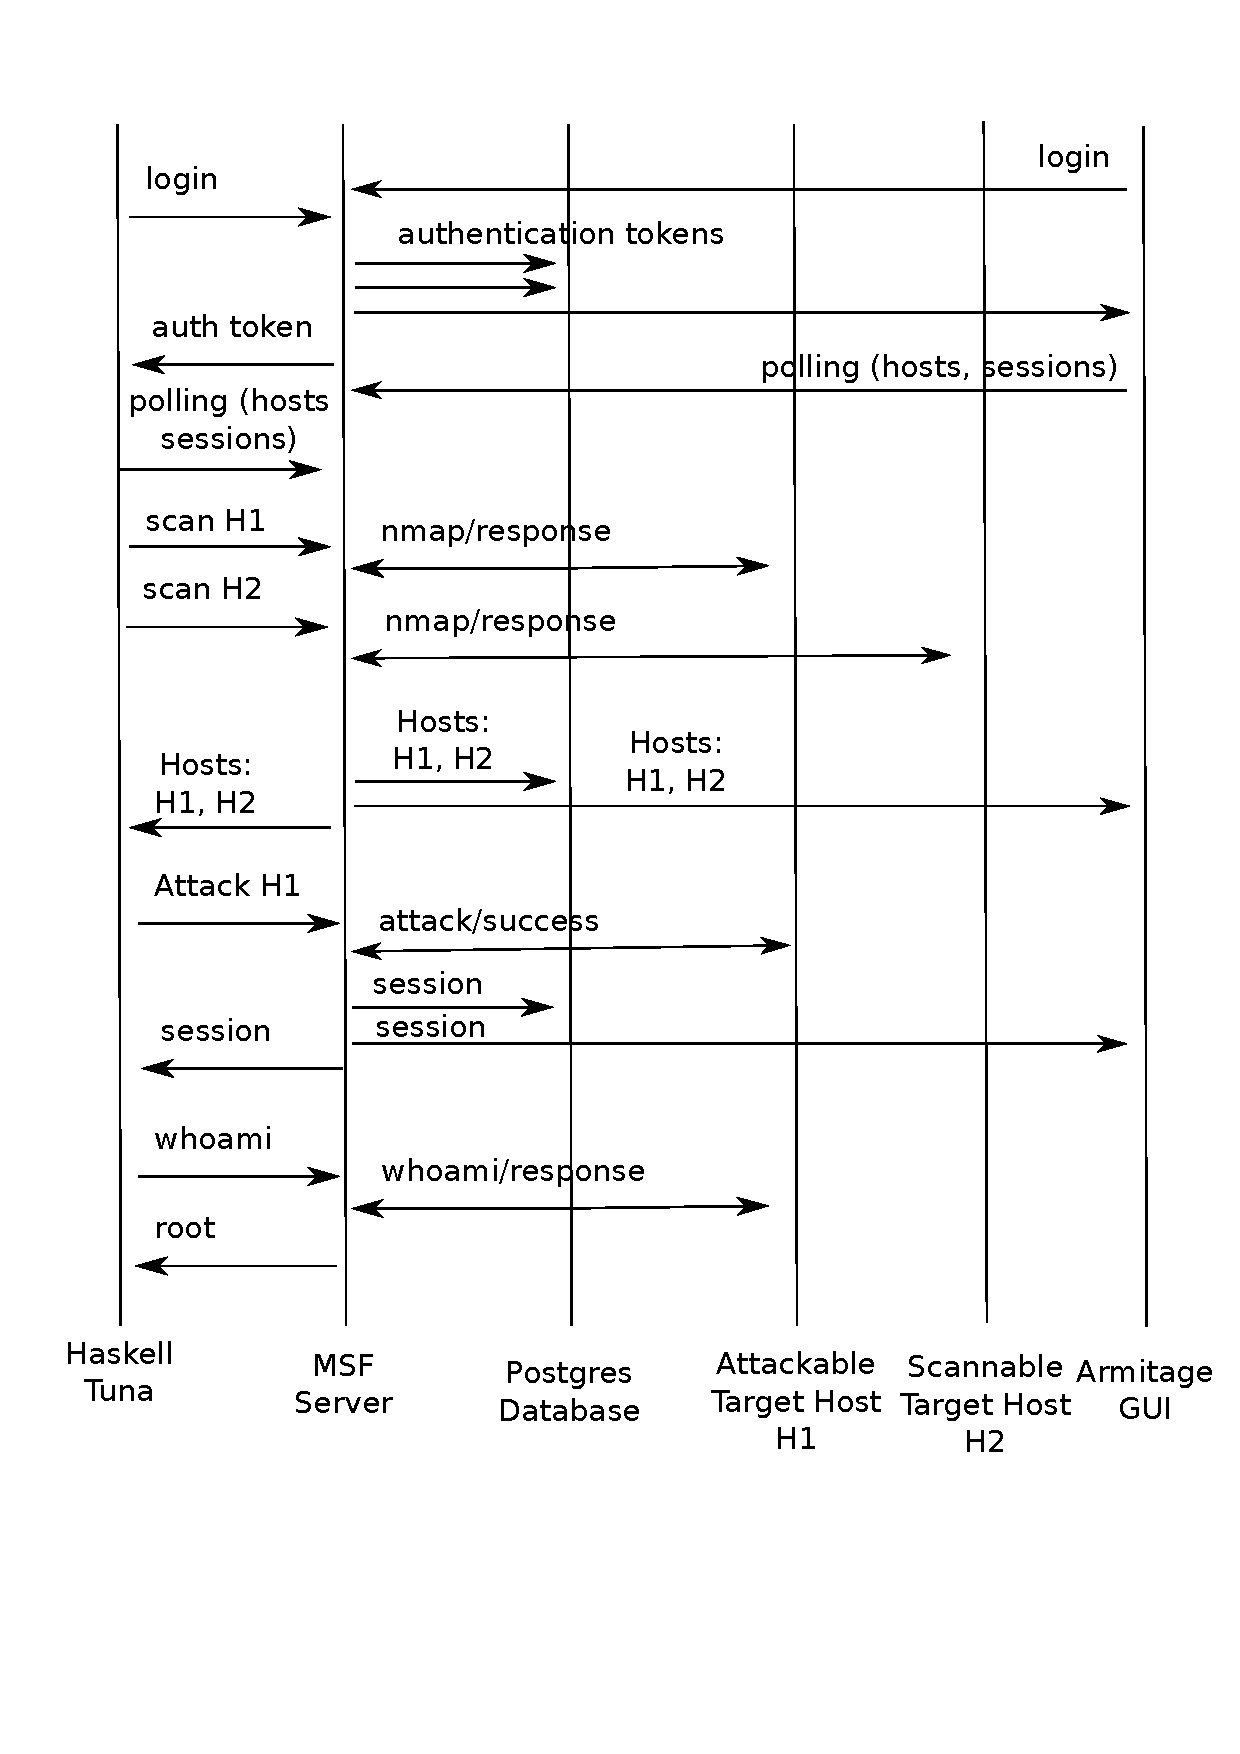
\includegraphics[scale=0.5]{serviceDiagram.pdf}
\end{figure}

%%%
% bibliography
%%%
%\bibliographystyle{siam}
%\bibliography{main}

\end{document}

